\documentclass[12pt]{article}

\usepackage[a4paper,margin=2.5cm]{geometry}
\usepackage{amsmath, amssymb, amsthm}
\usepackage{bm}
\usepackage{hyperref}
\usepackage{graphicx}
\usepackage{caption}
\usepackage{listings}
\usepackage{xcolor}
\usepackage{float}
\usepackage{placeins}
\graphicspath{{figures/}}

\lstdefinestyle{code}{
  basicstyle=\ttfamily\small,
  numbers=left,
  numberstyle=\tiny,
  numbersep=8pt,
  keywordstyle=\color{blue},
  commentstyle=\color{teal!70!black},
  stringstyle=\color{orange!70!black},
  showstringspaces=false,
  breaklines=true,
  frame=single,
  framerule=0.3pt,
  rulecolor=\color{black!15}
}
\lstset{style=code}

\title{Deep Deterministic Policy Gradient (DDPG) Tutorial}
\author{}
\date{\today}

\begin{document}
\maketitle

\section{Introduction}
Deep Deterministic Policy Gradient (DDPG) extends deterministic policy gradients to deep neural networks, combining actor-critic architectures with replay buffers and target networks. DDPG excels in continuous control tasks by learning a deterministic policy while stabilizing training through soft target updates.

\section{Theory and Formulas}
\subsection{Deterministic Policy Gradient}
For deterministic policy \(\mu_\theta(s)\) and critic \(Q_w(s,a)\), the objective gradient is
\begin{equation}
\nabla_\theta J(\theta) = \mathbb{E}_{s \sim \mathcal{D}}\big[ \nabla_a Q_w(s,a)\big|_{a=\mu_\theta(s)} \nabla_\theta \mu_\theta(s) \big].
\end{equation}
States are sampled from a replay buffer \(\mathcal{D}\), enabling off-policy learning.

\subsection{Critic Update}
The critic minimizes the temporal-difference loss with target networks \((\mu_{\theta^-}, Q_{w^-})\):
\begin{equation}
L(w) = \mathbb{E}_{(s,a,r,s')}\Big[ \big( r + \gamma Q_{w^-}(s', \mu_{\theta^-}(s')) - Q_w(s,a) \big)^2 \Big].
\end{equation}
Target networks are updated softly: \(\theta^- \leftarrow \tau \theta + (1-\tau)\theta^-\).

\subsection{Exploration Noise}
Because the policy is deterministic, exploration is introduced by adding noise \(\mathcal{N}_t\) to the action during data collection: \(a_t = \mu_\theta(s_t) + \mathcal{N}_t\). Ornstein-Uhlenbeck noise or Gaussian noise preserves temporal coherence.

\section{Applications and Tips}
\begin{itemize}
  \item \textbf{Robotics}: continuous torque control, manipulation, locomotion.
  \item \textbf{Industrial control}: optimize real-valued actuators with safety constraints.
  \item \textbf{Autonomous driving}: steering and throttle in simulation environments.
  \item \textbf{Best practices}: use large replay buffers, normalize observations, clip gradients, tune noise scale, and monitor critic loss for divergence.
\end{itemize}

\section{Python Practice}
The script \texttt{gen\_ddpg\_figures.py} trains a lightweight DDPG agent on a one-dimensional continuous control problem. It logs episode returns and the evolution of the deterministic policy across states.
\begin{lstlisting}[language=Python,caption={Excerpt from gen_ddpg_figures.py}]
# Critic update
q_pred = critic_w @ features(state, action)
q_target = reward + gamma * critic_target_w @ features(next_state, actor_target(next_state))
critic_w += critic_lr * (q_target - q_pred) * features(state, action)

# Actor update via deterministic policy gradient
grad_q = critic_grad(state, actor(state))
actor_theta += actor_lr * grad_q
\end{lstlisting}

\section{Result}
\begin{figure}[H]
  \centering
  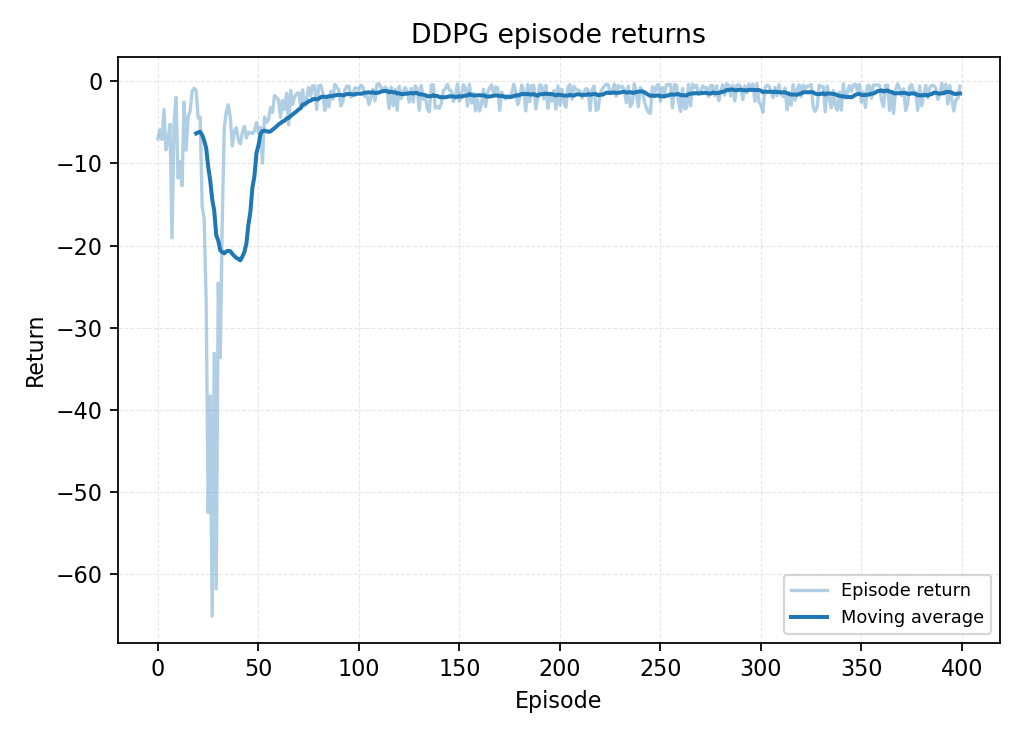
\includegraphics[width=0.8\linewidth]{ddpg_returns.png}
  \caption{DDPG training returns approaching the optimal control policy}
  \label{fig:ddpg_returns}
\end{figure}

\begin{figure}[H]
  \centering
  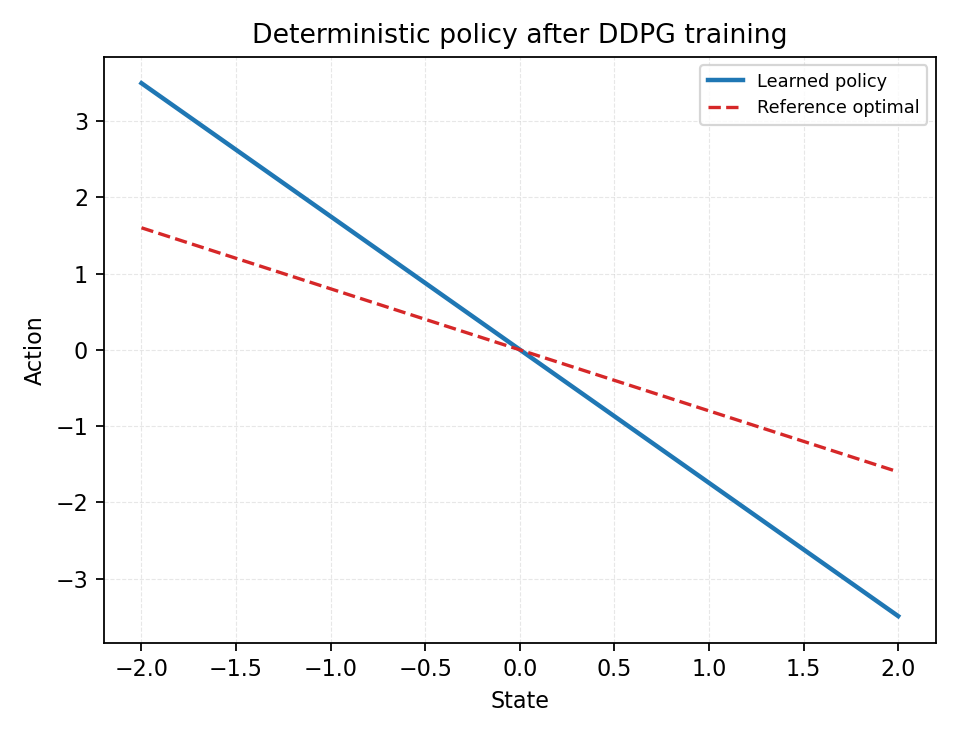
\includegraphics[width=0.82\linewidth]{ddpg_policy_trace.png}
  \caption{Learned deterministic policy across states compared to the optimal action}
  \label{fig:ddpg_policy_trace}
\end{figure}

\FloatBarrier
\section{Summary}
DDPG adapts deterministic policy gradients to deep function approximation using target networks and replay buffers for stability. Proper exploration noise, normalization, and critic monitoring are essential. The toy control example demonstrates improving returns and convergence of the actor toward optimal continuous actions.

\end{document}